\documentclass[tikz,11pt]{standalone}
\usepackage{newtxtext,newtxmath}
\usepackage{xifthen}

\usetikzlibrary{calc,positioning}

% Define sizes and parameters in cm
\def\width{10}
\def\height{6}

\def\levelsep{1.3}
\def\levelwidth{1.5}
\def\det{0.2}
\def\lrsep{3.5}

\tikzstyle{level}                = [very thick]

\begin{document}
    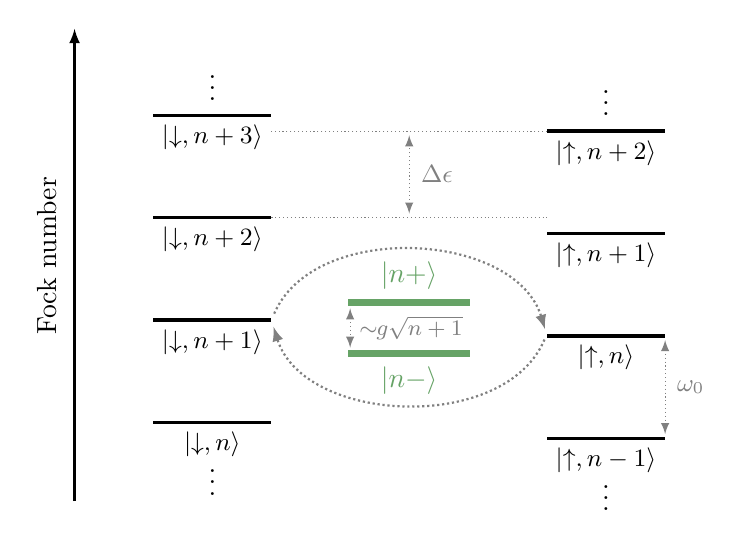
\begin{tikzpicture}[local bounding box=BB, every node/.style={outer sep=0pt}]
        % \path[draw,blue] (0,0) rectangle (\width,\height);
        \draw[-latex, thick] (0,0) -- (0,\height) 
              node[midway,left,label={[rotate=90]:Fock number}] {};


        \begin{scope}[shift={(1,1)}]
            \foreach \n in {0,...,3}
            {
                \draw[level] (0,{\n*\levelsep}) --++(\levelwidth,0)
                    node[inner sep=0pt,at end] (e\n) {}
                    node[midway,below]         (l\n) {\small $\left|\downarrow, n \ifthenelse{0 = \n}{}{+\n}\right\rangle$};
            }
            \node[below] at (l0) {\vdots};
            \node[above=1em] at (l3) {\vdots};
        \end{scope}

        \begin{scope}[shift={($(e0)+(\lrsep,-\det)$)}]
            \foreach \n in {-1,...,2}
            {
                \draw[level] (0,{(\n+1)*\levelsep}) --++(\levelwidth,0)
                    node[inner sep=0pt,at start] (w\n) {}
                    node[midway,below]           (r\n)
                    {\small $\left|\uparrow, n \ifthenelse{0 = \n}{}{\ifthenelse{-1 = \n}{-1}{+\n}}\right\rangle$}
                    node[inner sep=0pt, at end] (er\n) {};
            }

            \node[below] at (r-1) {\vdots};
            \node[above=1em] at (r2) {\vdots};

           \node[at={($(e1)!0.5!(w0)$)},fill=white,inner sep=0pt] (g) {};
            \draw[-latex,shorten <=2pt, shorten >=2pt,thick,black!50,densely dotted] (e1) to[bend left=70] (w0) edge[bend left=70]  (e1);

            \node[above=2ex,ultra thick,draw,fill,green!40!black!60,
                  minimum width=\levelwidth cm,
                  inner sep=0pt,outer sep=0pt,
                  label={[green!40!black!60,fill=white,inner sep=0pt,yshift=1ex]above:$|n+\rangle$}] (n+) at (g) {};
            \node[below=2ex,draw,fill,ultra thick,green!40!black!60,
                  minimum width=\levelwidth cm,
                  inner sep=0pt,outer sep=0pt,
                  label={[green!40!black!60,fill=white,inner sep=0pt,yshift=-1ex]below:$|n-\rangle$}] (n-) at (g) {};

            \draw[<->, >=latex, shorten <=2pt, shorten >=2pt, black!50,densely dotted] (n+.west)--(n-.west) node[midway,right] {\footnotesize $\sim\!\!g\sqrt{n+1}$};

        \end{scope}

        \draw[thin,gray,densely dotted] (e2.center) --++ (\lrsep,0) node[midway,inner sep=0pt] (du) {};
        \draw[thin,gray,densely dotted] (w2.center) --++ (-\lrsep,0) node[midway,inner sep=0pt] (dd) {};

        \draw[<->,>=latex,shorten <=1pt, shorten >=1pt,thin,gray,densely dotted] (du) -- (dd) node[midway,right=1ex,inner sep=0pt] {\small $\Delta\epsilon$};
        \draw[<->,>=latex,shorten <=1pt, shorten >=1pt,thin,gray,densely dotted] (er0) -- (er-1) node[midway,right=1ex,inner sep=0pt] {\small $\omega_0$};
    \end{tikzpicture}
\end{document}

